\documentclass[a4paper,11pt]{article}

\usepackage[T1]{fontenc}
\usepackage[utf8]{inputenc}
\usepackage{graphicx}
\usepackage{xcolor}

\renewcommand\familydefault{\sfdefault}
\usepackage{tgheros}
\usepackage[defaultmono]{droidmono}

\usepackage{amsmath,amssymb,amsthm,textcomp}
\usepackage{enumerate}
\usepackage{multicol}
\usepackage{tikz}

\usepackage{geometry}
\geometry{left=25mm,right=25mm,%
bindingoffset=0mm, top=20mm,bottom=20mm}


\linespread{1.3}

\newcommand{\linia}{\rule{\linewidth}{0.5pt}}

% custom theorems if needed
\newtheoremstyle{mytheor}
    {1ex}{1ex}{\normalfont}{0pt}{\scshape}{.}{1ex}
    {{\thmname{#1 }}{\thmnumber{#2}}{\thmnote{ (#3)}}}

\theoremstyle{mytheor}
\newtheorem{defi}{Definition}

% my own titles
\makeatletter
\renewcommand{\maketitle}{
\begin{center}
\vspace{2ex}
{\huge \textsc{\@title}}
\vspace{1ex}
\\
\linia\\
\@author \hfill \@date
\vspace{4ex}
\end{center}
}
\makeatother
%%%

% custom footers and headers
\usepackage{fancyhdr}
\pagestyle{fancy}
\lhead{}
\chead{}
\rhead{}
\lfoot{}
\cfoot{}
\rfoot{\thepage}
\renewcommand{\headrulewidth}{0pt}
\renewcommand{\footrulewidth}{0pt}
%

% code listing settings
\usepackage{listings}
\lstset{
    language=Python,
    basicstyle=\ttfamily\small,
    aboveskip={1.0\baselineskip},
    belowskip={1.0\baselineskip},
    columns=fixed,
    extendedchars=true,
    breaklines=true,
    tabsize=4,
    prebreak=\raisebox{0ex}[0ex][0ex]{\ensuremath{\hookleftarrow}},
    frame=lines,
    showtabs=false,
    showspaces=false,
    showstringspaces=false,
    keywordstyle=\color[rgb]{0.627,0.126,0.941},
    commentstyle=\color[rgb]{0.133,0.545,0.133},
    stringstyle=\color[rgb]{01,0,0},
    numbers=left,
    numberstyle=\small,
    stepnumber=1,
    numbersep=10pt,
    captionpos=t,
    escapeinside={\%*}{*)}
}

%%%----------%%%----------%%%----------%%%----------%%%

\begin{document}

\title{CS 426 Parallel Computing Project 2 Report}

\author{Bartu Atabek - 21602229}

\date{25/04/2020}

\maketitle

\section{Answers to The Questions}
\subsection{What is the difference in terms of parallelism, if any, between two strategies for approximating pi? Discuss in terms of data and task parallelism.}

First of all, in Part B we used only one strategy for approximating pi, which was the 'Monte Carlo Simulation'. It is used for both the parallel and the serial implementations. Since the question asks for the differences in term of data and task parallelism we cannot compare these two implementations. Although the parallel implementation uses data parallelism which means concurrent execution of the same task on each multiple computing cores. 

\subsection{What was your communication scheme, which MPI communication functions did you use and why.}

I used the collective communication features of the MPI while implementing the generic functions in Part A. Mainly I used \textbf{MPI\_Scatterv} with \textbf{MPI\_Gatherv}. I chose scatter and gather because in each function we needed to distribute the given array into chunks send them to different processes and gather their results in the end. Scatter as it can be known from its names takes an buffer and distributes it among the processes. I chose \textbf{MPI\_Scatterv} instead of \textbf{MPI\_Scatter} because the given array might not be divided equally perfectly to the number of processors. The same logic also applied for gather as well since map and filter returns the same number of elements they have distributed. As an exception, I used \textbf{MPI\_Gather} for the fold function because fold function reduces the given elements into a single result and since there can only be one result for each process I've used it.

\subsection{How MPI address space is used between processes? Are they threads, or are they different OS level processes? What would be in a distributed environment where you had many different computers connected together? Would function pointers, pointers to part of the code segment of virtual memory space, still work if we had a truly distributed environment.}

Basically on a single shared memory machine one can use POSIX threads and message queues but as pointed out, use of MPI and more advanced tools will save you time and allows better scaling. Because of this MPI address space used between processes as different OS level processes. In a truly distributed environment with many different computers connected together function pointers may or may not work depending on whether the address pointed by it is valid \& correct on each machine. For example a function pointer pointing to a part of the code segment of virtual memory space may not point to it's equivalent on another machine. However, since MPI distributes these code segments to each machine so that they could run the same code in parallel it should work.

\section{Results \& Discussion}
\subsection{Discuss your timing results and put your graphs according to number of processes.}

Although it was asked the reporting the results according to the number of processes the guidelines specified that the programs should only take one argument which is the number of experiments. The performance of the serial execution was compared with the parallel execution running with maximum available processes which was 4 for my computer, with respect to the number of experiments and the results with different number of processes between 1-3 are also reported.

First of all, for the results of running the parallel application with different number of processes as it can be seen from the figures below running the program with one process is equivalent to running in serial thus it's results are quite similar with the serial programs performance. As number of processes increase we first see an increase in the execution times. Because initially the array had locality and when we increased the number of processes we also added a communication overhead because data is distributed between all the processes and for small data such as 1000 items we are decreasing the locality when we increased the number of processes.

With respect to that, I observed that from the plots that the serial execution was faster in terms of run-time in all cases as it can be seen. However, when compared with the project 1 the results were improved. As for the reason of parallel program being slower could be explained with the following two key factors; parallel task granularity, communication overhead since load balancing among processes was done equally by scattering the data. By task granularity it is meant that the parallel tasks must be "big" enough to justify the overheads of parallelization. For the communication overhead reducing the amount of communication and synchronization between parallel tasks would improve the performance. Because of the data dependencies it was required to use \textbf{MPI\_Barrier} in order to wait for all processes to come to the same point which may blocked some tasks to proceed asynchronously.

\begin{figure}[!htb]
    \centering
    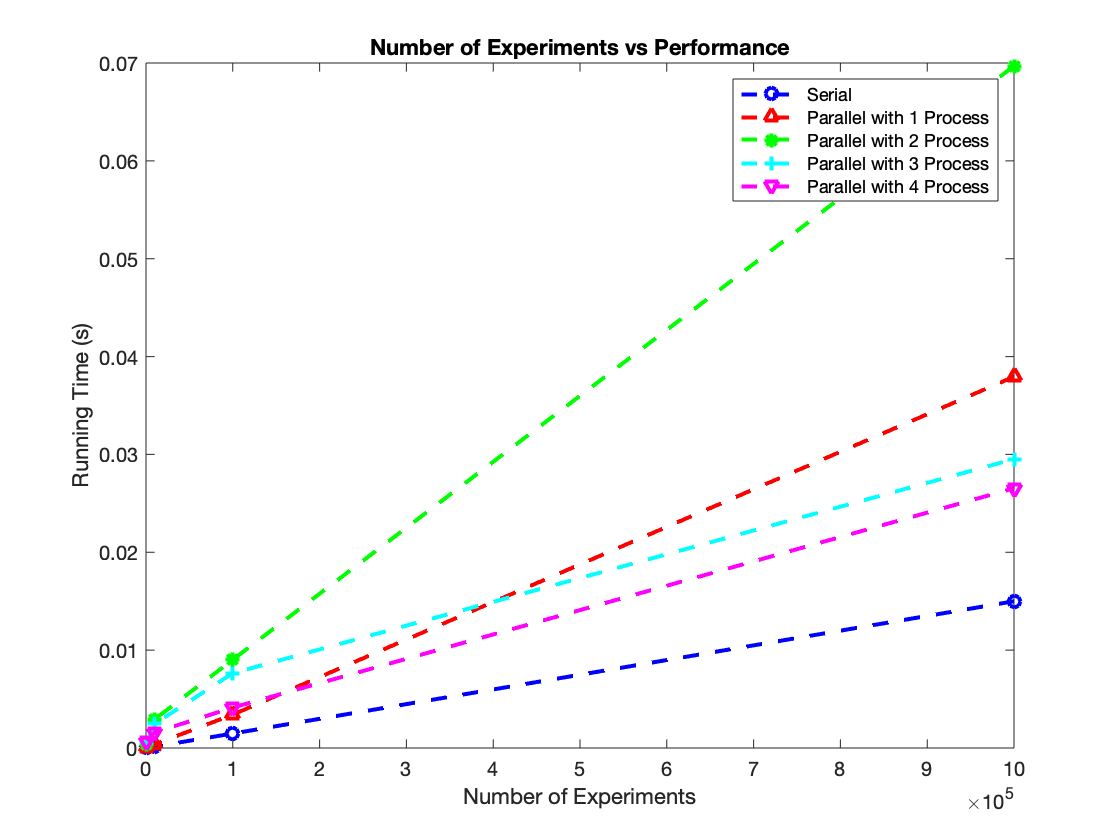
\includegraphics[width=0.75\textwidth]{figure1}
    \caption{Run-time comparison of Pi estimation programs written in serial and parallel accordingly with different number of experiments i.e.  1000,10000,100000,1000000 where parallel execution was tested with 1,2,3,4 processes.}
\end{figure}

\begin{figure}[!htb]
    \centering
    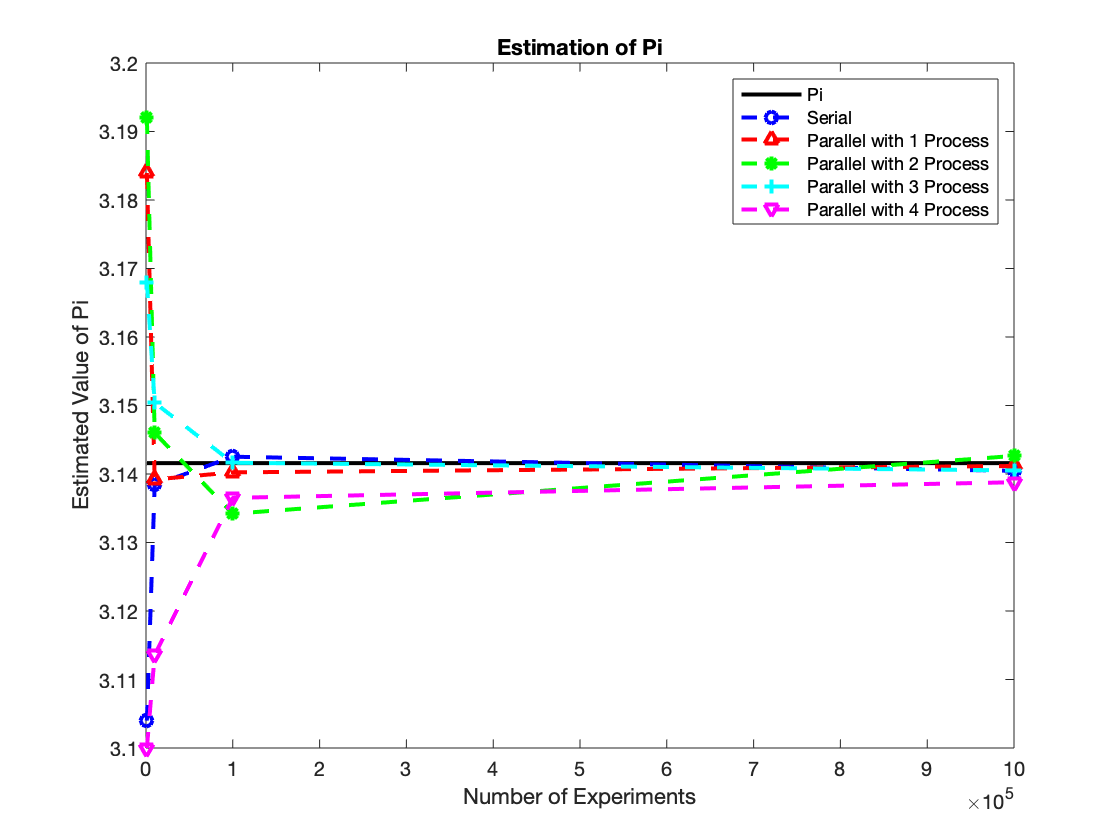
\includegraphics[width=0.75\textwidth]{figure2}
    \caption{Value estimation of Pi obtained by simulating 1000,10000,100000,1000000 experiments using Monte Carlo Simulation in serial and parallel executions compared with the real value of Pi where parallel execution was tested with 1,2,3,4 processes.}
\end{figure}
\end{document}
